\chapter{Design}\label{Design}

\section{Desired Work-cell}

\begin{figure}[h]
    \centering
    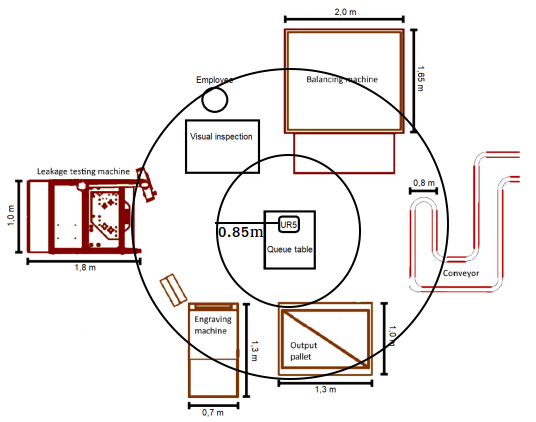
\includegraphics[width=9cm]{Design/Work_cell_3.png}
    \caption{work-cell with measurements and reach}
    \label{fig:workcellMR}
\end{figure}

When looking at \ref{fig:workcellMR}, a systematic work-cell is presented. But the important thing of a work-cell is its flow.\\
Here is some sections about what is needed of the ideal work-cell.

\subsection{Dexterous work-space}

The work-space which a manipulator works within can be described as a radius which the point of the end-effector can reach.\\
The Dexterous work-space is a more intelligent way of the robot to decide which points in arbitrary orientation, can be reached \cite{Dexterous}.\\
The reason that the dexterous work-space is considered a solution to the work-cell, is that the kinematic restrains can be included, so that the trajectories of the manipulator wont freeze or go in lock down.\\


\subsection{Safety}

The safety in the work-cell is important, since it helps prevent eventual accidents that might be avoidable with some safety measures. The work-cell also has to comply to the required legal safety regulations.\\
One safety measure that could be beneficial in the work-cell is a "light curtain" sensor, see\ref{SafetyDevices}.
When a light beam from the light curtain is broken, it can signal the UR5 inside the work-cell to slow down.\\
The light curtain can be placed around the work-cell, so it is triggered whenever someone enters the work-cell. This allows the production to continue, while making the work-cell more safe for anyone entering the work-cell \ref{SafetyDevices}.\\
To further improve the safety, a LIDAR sensor could be used.
LIDAR is a common sensor that can scan an environment at a variety of ranges,see \ref{SafetyDevices}.
The LIDAR sensor can be used to detect, when a person enters the proximity of the UR5 within the work-cell. When the LIDAR detects something, it can signal the UR5 to stop completely. This can reduce the risk of injury further, since it could be dangerous for people to be struck with a rotor, even at low speeds.\\
The above safety precautions would increase the work-cell safety, while still allowing some progress to be made, when there are people in the work-cell.\\

\subsection{Safety Requirements}

The most important solution for the safety of the work-cell, is the ISO 10218-2:2011, see \ref{ISO2}.\\
When installing a new robot for a production line, some standards is required. These standards of the ISO can present which of the areas needed to be acted upon.\\

\subsection{Placement Sensors}

To ensure the work-flow some intelligent placement sensors must be implemented. Some of the possible solutions are chosen:\\

\begin{itemize}
    \item LIDAR
    \item Photocell sensors
    \item Depth sensing camera
\end{itemize}
\\
The LIDAR is a sensor that gives a 3D view, and can be used for the robot to tell the different object apart, and give an overview of the work-cell, see \ref{ref:PlacementS}.\\
These signals can be used for the cobot to get a better work-flow and also determine objects from each other.\\
\\
The photocell sensors can be used for a quicker work-flow, since it will detect the rotors when they are in the correct place to be picked up, see \ref{ref:PlacementS}.\\
\\
Depth sensing cameras can determine the distance from end-effector to the desired object, see \ref{ref:PlacementS}. This can be used to derive the distance from the certain machine where the rotor has to be placed.\cu

\section{Desired Robot}\label{IdealRobot}

The desired robot to have inside the work-cell, is intelligent, fast and can decide the next trajectory without any hesitation. Its size is optimized to fit the given case, to work at the most effective speed possible.\\

\subsection{Desired speed}

The robot has 6 tasks it needs to complete within 26 seconds. This means that the slowest possible speed it has to have per translation to other machines, while delivering the rotor, is 26 divided by 6, which will give the manipulator an average of 4.33 seconds to carry out each task.\\
Taking the visual inspection in consideration, the number has to be lower when translating from the machines. The person inspecting might need something close to 5 seconds. Taking that into consideration a new formula for the speed of the cobot can be found.\\

\begin{equation}
    26 = 5 + 6 \times b \Rightarrow b = \frac{21}{6}\\
\end{equation}

\begin{equation}
    b = \frac{21}{6} \Rightarrow b = \frac{7}{2}\\
\end{equation}

\begin{equation}
    b = \frac{7}{2} \Leftrightarrow  b = 3.5 sec\\
\end{equation}
\\
5 seconds in one station means that the other stations needs to be cut down with 0.2 seconds each.\\
So the optimal speed for translations would be 3.5 seconds.\\

\subsection{Desired reach}

The manipulator must be able to reach all pick and place points, without having to move its base. Given the work-cell design, this means the robot will need a reach of 2 meters. \\
\begin{figure}[H]
    \centering
    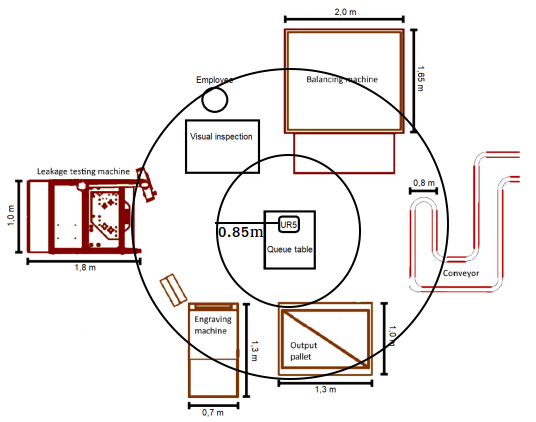
\includegraphics[width=8cm]{Design/Work_cell_3.png}
    \caption{Work-cell with measurements and reach}
    \label{fig:workcell}
\end{figure}
\\
This desired reach could also be accomplished by changing the setup to use 2 manipulators, see figure \ref{fig:workscell2arms}. By doing it this way, the 2 robots would only need one place where their reach overlap, so they can both pick and place the rotors on a buffer table. This would also require additional programming, which should prevent the two robots from hitting each other.\\

\begin{figure}[H]
    \centering
    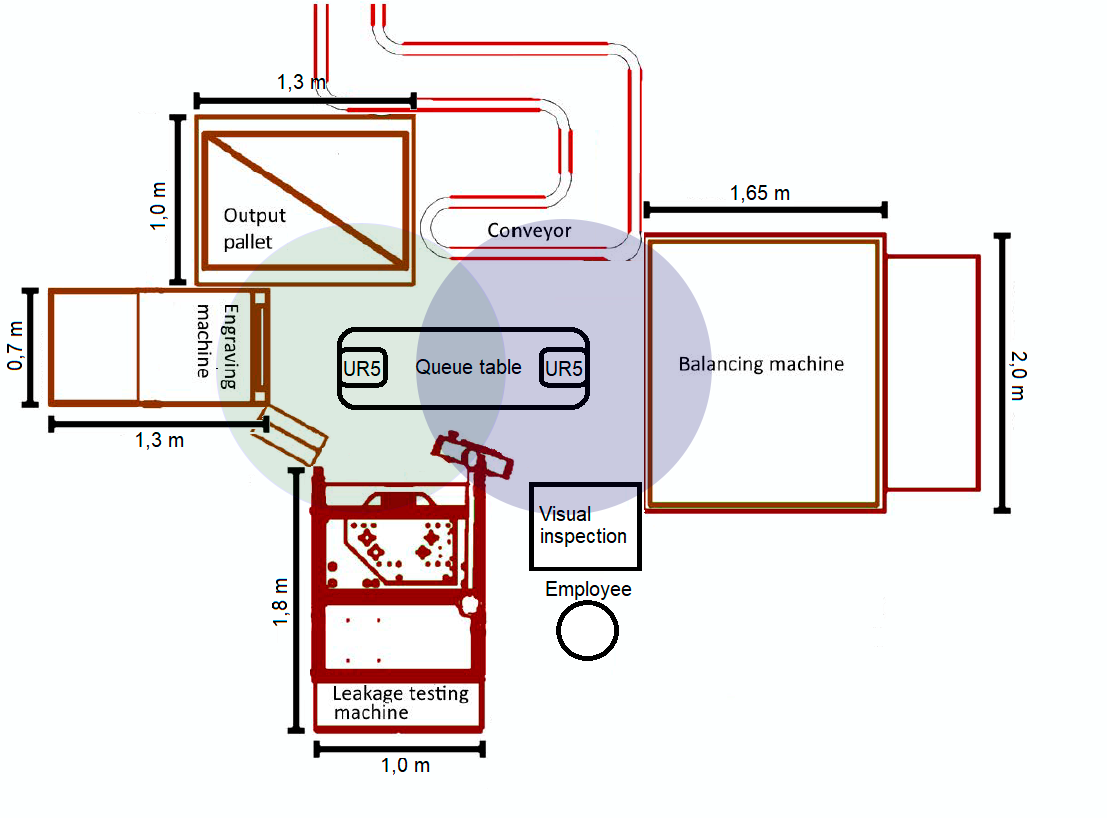
\includegraphics[width=.5\textwidth]{Design/Work_cell_8.PNG}
    \caption{Work-cell design with 2 robots}
    \label{fig:workscell2arms}
\end{figure}

\begin{figure}[H]
  \centering
  \begin{minipage}[b]{0.45\textwidth}
    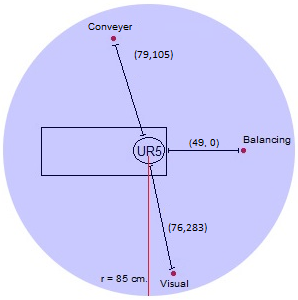
\includegraphics[width=\textwidth]{Design/workcell_1_polar.png}
    \label{fig:position}
  \end{minipage}
  \hfill
  \begin{minipage}[b]{0.45\textwidth}
    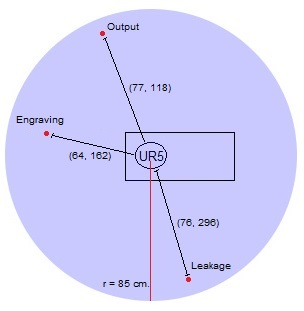
\includegraphics[width=\textwidth]{Design/polar.jpg}  
    \label{fig:velocity}
  \end{minipage}
  {Work-cell first and second part ,with polar coordinates and reach to suited the reach of the UR 5.}
\end{figure}
%Flowchart 1:
\begin{tikzpicture}[node distance=2cm]

%Primary nodes:
\node (start) [startstop] {Rotor arrives on conveyer/queue table};
\node (dec1) [decision, below of=start, yshift=-2.5cm] {Has this rotor been balance tested?};
\node (dec2) [decision, right of=dec1, xshift=3.2cm] {Is the balancing
machine empty?};
\node (pro1) [process, right of=dec2, xshift=3.1cm] {Move the rotor to balancing machine};
\node (out1) [io, below of=pro1, yshift=-3cm] {Balancing complete};
\node (dec3) [decision, below of=dec1, yshift=-6cm] {Has this rotor been visually inspected?};
\node (dec4) [decision, right of=dec3, xshift=3.2cm] {Is visual inspection available?};
\node (pro2) [process, right of=dec4, xshift=3.1cm] {Move the rotor to visual inspection};
\node (out2) [io, below of=pro2, yshift=-3cm] {Visual inspection complete};
\node (stop) [startstop, below of=dec3, yshift=-5cm] {Move rotor to queue table};

%Primary arrows:
\draw [arrow] (start) -- (dec1);
\draw [arrow] (dec1) -- node[anchor=south] {no} (dec2);
\draw [arrow] (dec1) -- node[anchor=west] {yes} (dec3);
\draw [arrow] (dec2) -- node[anchor=south] {yes} (pro1);
\draw [arrow] (pro1) -- (out1);
\draw [arrow] (dec3) -- node[anchor=south] {no} (dec4);
\draw [arrow] (dec3) -- node[anchor=west]  {yes} (stop);
\draw [arrow] (dec4) -- node[anchor=south] {yes} (pro2);
\draw [arrow] (pro2) -- (out2);

%dec2, dec4 -> start:
\node (gui1) [Guidebox, left of=pro1, xshift=-11cm] {};
\node (gui2) [Guidebox, below of=gui1, yshift=-0.85cm] {};
\node (gui6) [Guidebox, left of=pro2, xshift=-11cm] {};
\node (gui7) [Guidebox, below of=gui6, yshift=-0.85cm] {};

%Below dec2:
\node (gui3) [Guidebox, right of=gui2, xshift=5.9cm] {};
\node (gui4) [Guidebox, below of=gui3, yshift=1.9cm] {};
\node (gui5) [Guidebox, right of=gui3, xshift=-1.9cm] {};
\draw [arrow] (dec2) -- node[anchor=west] {no} (gui4);
\draw [arrow] (gui5) -- (gui2);

%Below dec4:
\node (gui8) [Guidebox, right of=gui7, xshift=5.9cm] {};
\node (gui9) [Guidebox, below of=gui8, yshift=1.9cm] {};
\node (gui10) [Guidebox, right of=gui8, xshift=-1.9cm] {};
\draw [arrow] (dec4) -- node[anchor=west] {no} (gui9);

%Line to start:
\node (gui11) [Guidebox, above of=gui1, yshift=2.55cm] {};
\node (gui12) [Guidebox, above of=gui11, yshift=-1.9cm] {};
\node (gui13) [Guidebox, left of=gui11, xshift=1.9cm] {};
\node (gui16) [Guidebox, below of=gui7, yshift=1.9cm] {};
\node (gui17) [Guidebox, left of=gui7, xshift=1.9cm] {};
\draw [arrow] (gui10) -- (gui17);
\draw [arrow] (gui16) -- (gui12);
\draw [arrow] (gui13) -- (start);

%out1, out2 -> dec3, stop:
\node (gui14) [Guidebox, above of=dec3, yshift=1cm] {};
\draw [arrow] (out1) -- (gui14);
\node (gui15) [Guidebox, above of=stop, yshift=-0cm] {};
\draw [arrow] (out2) -- (gui15);

%Caption:
\node (cap1) [Caption, below of=dec4, yshift=-7cm] {This flowchart shows the process performed by the first UR5 in the work-cell.};

\label{fig:first-part}
\end{tikzpicture}


%Flowchart 2:
\begin{tikzpicture}[node distance=2cm]

%Primary nodes:
\node (start) [startstop] {Rotor arrives on queue-table};
\node (dec1) [decision, below of=start, yshift=-2.5cm] {Has this rotor been leak tested?};
\node (dec2) [decision, right of=dec1, xshift=3.2cm] {Is the leak testing
machine empty?};
\node (pro1) [process, right of=dec2, xshift=3.1cm] {Move the rotor to leak testing machine};
\node (out1) [io, below of=pro1, yshift=-3cm] {Leak testing complete};
\node (dec3) [decision, below of=dec1, yshift=-6cm] {Has this rotor been engraved?};
\node (dec4) [decision, right of=dec3, xshift=3.2cm] {Is the engraving
machine empty?};
\node (pro2) [process, right of=dec4, xshift=3.1cm] {Move the rotor to engraving machine};
\node (out2) [io, below of=pro2, yshift=-3cm] {Engraving complete};
\node (stop) [startstop, below of=dec3, yshift=-5cm] {Move rotor to output pallet};

%Primary arrows:
\draw [arrow] (start) -- (dec1);
\draw [arrow] (dec1) -- node[anchor=south] {no} (dec2);
\draw [arrow] (dec1) -- node[anchor=west] {yes} (dec3);
\draw [arrow] (dec2) -- node[anchor=south] {yes} (pro1);
\draw [arrow] (pro1) -- (out1);
\draw [arrow] (dec3) -- node[anchor=south] {no} (dec4);
\draw [arrow] (dec3) -- node[anchor=west]  {yes} (stop);
\draw [arrow] (dec4) -- node[anchor=south] {yes} (pro2);
\draw [arrow] (pro2) -- (out2);

%dec2, dec4 -> start:
\node (gui1) [Guidebox, left of=pro1, xshift=-11cm] {};
\node (gui2) [Guidebox, below of=gui1, yshift=-0.85cm] {};
\node (gui6) [Guidebox, left of=pro2, xshift=-11cm] {};
\node (gui7) [Guidebox, below of=gui6, yshift=-0.85cm] {};

%Below dec2:
\node (gui3) [Guidebox, right of=gui2, xshift=5.9cm] {};
\node (gui4) [Guidebox, below of=gui3, yshift=1.9cm] {};
\node (gui5) [Guidebox, right of=gui3, xshift=-1.9cm] {};
\draw [arrow] (dec2) -- node[anchor=west] {no} (gui4);
\draw [arrow] (gui5) -- (gui2);

%Below dec4:
\node (gui8) [Guidebox, right of=gui7, xshift=5.9cm] {};
\node (gui9) [Guidebox, below of=gui8, yshift=1.9cm] {};
\node (gui10) [Guidebox, right of=gui8, xshift=-1.9cm] {};
\draw [arrow] (dec4) -- node[anchor=west] {no} (gui9);

%Line to start:
\node (gui11) [Guidebox, above of=gui1, yshift=2.55cm] {};
\node (gui12) [Guidebox, above of=gui11, yshift=-1.9cm] {};
\node (gui13) [Guidebox, left of=gui11, xshift=1.9cm] {};
\node (gui16) [Guidebox, below of=gui7, yshift=1.9cm] {};
\node (gui17) [Guidebox, left of=gui7, xshift=1.9cm] {};
\draw [arrow] (gui10) -- (gui17);
\draw [arrow] (gui16) -- (gui12);
\draw [arrow] (gui13) -- (start);

%out1, out2 -> dec3, stop:
\node (gui14) [Guidebox, above of=dec3, yshift=1cm] {};
\draw [arrow] (out1) -- (gui14);
\node (gui15) [Guidebox, above of=stop, yshift=-0cm] {};
\draw [arrow] (out2) -- (gui15);

%Caption:
\node (cap1) [Caption, below of=dec4, yshift=-7cm] {This flowchart shows the process performed by the second UR5 in the work-cell.};

\end{tikzpicture}






\subsection{Desired sensors}

The robot should be able to identify humans, and collisions must be risk free, and not disrupt the work-flow. Optimally, the robot should also be able to identify what object it is holding, and if it is damaged or not. Additionally, the robot must be able to place the rotors correctly in the machines, using a depth sensing camera. \ref{depthcam}\\
The robot should be able to register whether or not it has picked up a rotor. This can be done by using a pressure sensor.\\ 

\subsection{Max payload}
The robot manipulator must be able to lift more then  the combined weight of the L40 rotor, aswell as the end-effector tool to move the rotor.\\


%\ref{workscell2arms}. this ref is not linking to anything??
%The robot must be able to lift the L40 rotor given in the case, which weighs 645 grams. The end-effector must also be able to grab it, without the risk of dropping it. The rotor is 190mm long, and 90mm wide at its widest point. The manipulator must also be able to support the[width=8cm] weight when the arm is fully stretc\ref{workscell2arms}

\section{Conclusion} 

looking into what an optimal layout for the work-cell could be, with respect to the above problem-analysis, it is considered that these items are desirable for the work-cell.\\
A desired robot has been specified using the different requirements from the previous chapters. In terms of the desired speed, it was concluded that the robot should be able to complete each task in 3,5 seconds or less.\\
It was also concluded that one of the following solutions would be required for the robot to reach everything in the work-cell: 
\begin{itemize}
    \item The chosen robot would have a reach of at least 2 meters.
    \item 2 robots would be in the work-cell at the same time. 
    \item The robot would have a movable base. 
\end{itemize} 
Additionally, the desired sensors in the work-cell should be able to identify humans, detect the rotor which the robot is holding, detect the orientation of this rotor, and whether it is damaged. The sensors should also allow the robot in the work-cell to place the rotors correctly into each machine. It is also concluded that the robot should lift a payload greater than the end-effector and the L40 rotor combined.\\

\chapter{Trajectories}\label{ch:kinematics}

In this chapter there will be described some mathematical expression of manipulators in general and for the UR5, and the trajectory planning of the UR5.

\section{Denavit-Hartenberg}

In order to enable the UR5 on the flexible workstation to locate itself and its surroundings within a space, the DH (Denavit-Hartenberg) method is used.\\ 
The DH method can be used to compute every frame into parameters.\\
These descriptions of the system can be used to translate every point and every movement of the robotic manipulator, with the help of forward kinematic.\\
Initially the start is to locate all of the coordinate systems, as seen in \ref{table:1}.\\ 


\begin{itemize}
    \item ${a_{i-1}}$= The distance from ${Z_{i-1}}$ to ${Z_{i}}$ measured along ${X_{i-1}}$
    \item ${\alpha_{i-1}}$ = The angel between ${Z_{i-1}}$ to ${Z_{i}}$ measured about ${X_{i-1}}$
    \item ${d_{i}}$ = The distance from ${X_{i-1}}$ to ${X_{i}}$ measured along ${Z_{i}}$
    \item ${\theta_{i-1}}$ = The angel between ${X_{i-1}}$ to ${X_{i}}$ measured about ${Z_{i}}$
\end{itemize}

\\
Then the angles and the distance from each coordinate system is computed and set in to a table as seen in \ref{fig:DH-Table}.

\begin{figure}[h!]
    \centering
    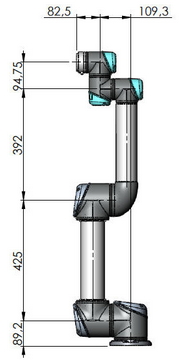
\includegraphics[scale=0.79]{Design/UR5measure.png}
    \caption{UR5 to describing DH-parameters \cite{DH}} 
    \label{fig:DH-Table} 
\end{figure}

%\begin{table}[h!]
%\centering
%\begin{tabular}{||c c c c c||} 
% \hline
% i & \alpha_{i-1} & a_{i-1} & d_{i} & \theta_{i} \\ [0.5ex] 
% \hline\hline
% 1 & 0 & 0  & 0     & \theta_{1} \\ 
% 2 & 0 & l_{1} & 0 & \theta_{2} \\
% 3 & 0 & l_{2} & 0 & \theta_{3} \\[1ex]
% \hline
%\end{tabular}
%\caption{DH-Table}
%\label{table:DH-table}
%\end{table}
\\
As seen in \ref{fig:DH-Table},the coordinate systems is used to trace every step of each axis.\\
Starting from left to right at the top of the table, the $\alpha-1$ is used to compute the differences of the angles between $Z_{i}$ and $Z_{i-1}$, which is 0, due to the fact that they keep the same angle from $Z_{i}$  to $Z_{i-1}$.\\
It can also be seen from the table that the distance between $Z_{i}$ and $Z_{i-1}$ is Length2, since they are parallel to each other.\\ 
The distance between $X_{i-1}$ and $X_i$ is 0 since they cross each other on the perpendicular line, which means that in that point the new coordinate system should be placed.\\

\begin{table}[h!]
\centering
\begin{tabular}{||c c c c c||} 
 \hline
 i & $\alpha_{i-1}$ & $a_{i-1}$ & $d_{i}$ & $\theta_{i}$ \\ [0.5ex] 
 \hline 
 \hline
 1 & 0 & 0 & 89.20 & $\theta_{1}$ \\ 
 2 & 90 & 0 & 0 & $\theta_{2}$+180 \\
 3 & 0 & 425 & 0 & $\theta_{3}$ \\
 4 & 0 & 392.43 & 109 & $\theta_{4}$ \\
 5 & -90 & 0 & 93.65 & $\theta_{5}$ \\ 
 6 & 90 & 0 & 82 & $\theta_{6}$+180\\[1ex] 
 \hline
\end{tabular}
\caption{DH-parameters for the UR5, using \cite{DHPar} as measurement.}
\label{table:1}
\end{table}

\section{Angle axis representation}

There are different ways to represent rotation, there is the roll, pitch and yaw. The best way to understand this is by showing a visual representation \ref{fig:rpy-rep}
\begin{figure}[H]
    \centering
    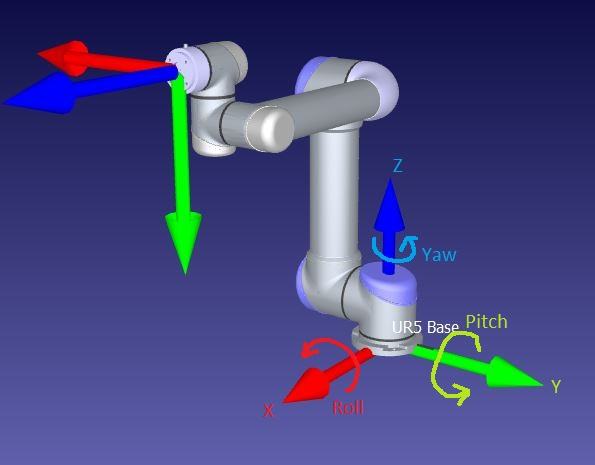
\includegraphics[width=\textwidth]{Design/UR5RPY.JPG}
    \caption{a representation of roll,pitch and yaw\cite{CHRobotics}}
    \label{fig:rpy-rep}
\end{figure}

where roll is a rotation around the X axis, pitch is a rotation around the Y axis and yaw is a rotation around the Z axis\cite{JohnC}.\\
The way that rotations are represented for the UR 5 is called angle axis, the way to understand this is by having specific vectors for a certain rotation see figure \ref{fig:rpy-rep}. The vector is used as an axis that rotation is going about\cite{JohnC}.

\subsection{Robot singularities}
The American National Standard for Industrial Robots and Robot systems, define singularities as "\textit{a condition caused by the collinear alignment of two or more robot axes resulting in unpredictable robot motion and velocities}\cite{3Sing}".\\
3 types of singularities can happen \cite{3Sing}.

\paragraph{Wrist:} When 2 of the axis of the robots wrist joints, are parallel with each other, it can cause them to spin 180 degrees at an infinity velocity.
\paragraph{Shoulder:} When the wrist aligns with the joint 1 axis, it will cause the shoulder part of the robot to spin 180 degrees in an instant, to try and follow the motion, same will happen if joint 1 and 6 line up with each other.
\paragraph{Elbow:} Unlike the other 2, this singularity instead locks the elbow in a stretched position, and happens when the center of the robot's wrist ends up on the same plane as joints 2 and 3, and will look like the arm is fully stretched, and tried to reach too far.

\section{Forward Kinematics}
The general idea behind forward kinematics, is that when given the joint angles from a manipulator as input, it is possible to compute the position and orientation for the end-effector as an output. This can then be used in a simulation of any manipulator.\\
Below are the general transformation matrices derived in Introduction to Robotics \cite{JohnC},this can be used to derive each joint transformation. In this matrix, the DH-parameters is used so the mechanical design of the manipulator is a fixed value and the angle values is a variable.\\
\begin{equation}
\centering
_i^{i-1}T = \begin{bmatrix} Cos(\theta_i) & -Sin(\theta_i) & 0 & a_{i-1}\\
Sin(\theta_i)*Cos(\alpha_{i-1}) & Cos(\theta_i)*Cos(\alpha_{i-1}) & -Sin(\alpha_{i-1}) & -Sin(\alpha_{i-1})*d_i\\
Sin(\theta_i)*Sin(\alpha_{i-1})& Cos(\theta_i)*Sin(\alpha_{i-1}) & Cos(\alpha_{i-1}) & Cos(\alpha_{i-1})*d_i \\
0 & 0 & 0 & 1\\ \end{bmatrix}
    \caption{Caption}
    \label{fig:my_label}
\end{equation}
\\


\begin{equation}
\centering
_0^BT = \begin{bmatrix} 1&0&0&0\\0&1&0&0\\0&0&1&0\\ 0&0&0&1\end{bmatrix}
    \caption{Caption}
    \label{fig:tb0}
\end{equation}

\begin{equation}
\centering
_1^0T = \begin{bmatrix} Cos(\theta_1)&-Sin(\theta_1)&0&0\\Sin(\theta_1) & Cos(\theta_1)&0&0\\0&0&1& d_1\\0&0&0&1 \end{bmatrix}
    \caption{Caption}
    \label{fig:t01}
\end{equation}

\begin{equation}
\centering
_2^1T = \begin{bmatrix} Cos(\theta_2)&-Sin(\theta_2)&0&0\\
0&0&-1&0\\Sin(\theta_2)& Cos(\theta_2)&0&0\\0&0&0&1\end{bmatrix}
    \caption{Caption}
    \label{fig:t12}
\end{equation}

\begin{equation}
\centering
_3^2T = \begin{bmatrix} Cos(\theta_3)&-Sin(\theta_3)&0&a_2\\
Sin(\theta_3)&Cos(\theta_3)&0&0\\0&0&1&0\\0&0&0&1\end{bmatrix}
    \caption{Caption}
    \label{fig:t23}
\end{equation}
\begin{equation}
\centering
_4^3T = \begin{bmatrix} Cos(\theta__4)&-Sin(\theta_4)&0&a__3\\
Sin(\theta_4)&Cos(\theta_4)&0&0\\0&0&1& d_4\\0&0&0&1\end{bmatrix}
    \caption{Caption}
    \label{fig:t34}
\end{equation}

\begin{equation}
\centering
_5^4T = \begin{bmatrix} Cos(\theta_5)&-Sin(\theta_5)&0&0\\
0&0&1&d_5\\-Sin(\theta_5)&-Cos(\theta_5)&0&0\\0&0&0&1\end{bmatrix}
    \caption{Caption}
    \label{fig:t45}
\end{equation}

\begin{equation}
\centering
_6^5T = \begin{bmatrix} Cos(\theta_6)&-Sin(\theta_6)&0&0\\https://www.sharelatex.com/project/5a829b040d7aa54a74a65ba0
0&0&-1&-d_6\\Sin(\theta_6)&Cos(\theta_6)&0&0\\0&0&0&1\end{bmatrix}
    \caption{Caption}
    \label{fig:t56}
\end{equation}

\\
Inserting arbitrary angels in each joint transformation matrices the position and orientation can be computed.
This can be done by using the following formula \ref{fig:tdot}, and using the dot-product on each transformation matrix, up to the desired point.\\
\begin{equation}
    _N^0 T\; =\ _1^0T\  _2^1T\  _3^2T\  _4^3T\  .........\  _N^{N-1}T\\
\caption{Caption}
    \label{fig:tdot}
    \end{equation}\\
Kinematics can be used to form an internal picture in a cartesian space  of the robot movements, and help understanding and explaining it.\\
This is useful when working with not only manipulators, but also animations in movies and video games, or any other movement where multiple joints are used.\\
\paragraph{Transformation matrix}
For calculating a transformation matrix to be used when testing,the DH-parameters and some angle values had to be used. The group choose 10, 20, 30, 40, 50 60, when inserting them into the previous mention matrices from \ref{fig:t01} to \ref{fig:t56} and using the dot-product as in \ref{fig:tdot}. The group derived at this matrix
\begin{equation}
\centering
_6^0 T = \begin{bmatrix} -0.786357421476564 & -0.607604499854991 & 0.111618896951653 & -521.411309306909\\-0.527586986670956 & 0.566511110959708 & -0.633022221383129 & -256.142081438594\\
0.321393804908450 & -0.556670399249454 & -0.766044443341916 & -419.593026103387 \\
0 & 0 & 0 & 1\\ \end{bmatrix}
    \caption{Caption}
    \label{fig:transfomationM}
\end{equation}\\

\section{Inverse Kinematics}
Inverse kinematics is used to compute the joint angles from a given position and orientation of an object \cite{JohnC}. The inverse kinematic can be set up from two aspects, one is the geometric way and the other is an algebraic solution, the one the team is using is the algebraic solution, where the inverse kinematics is set up in Maple, a math computer program, where it makes it possible to be used later in computing the trajectory of the manipulator.\\

\subsection{Finding the theta's}
These steps are inspired by \cite{Rasmus}.
Further calculations can be seen in a "maple" document attached with the document.\\

\paragraph{Step 1:} Use the transformation matrix \ref{fig:transfomationM}.This transformation matrix will be used to calculate the angles the UR 5 will have at this specif rotation and position.\\


\paragraph{Step 2:} Find $^5P_0$ this gives information on the position with respect from frame 5 to base.This gives two 90 degree triangle see \ref{fig:rasmus1}.\\

\begin{figure}[H]
    \centering
    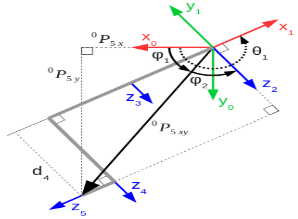
\includegraphics[scale=0.79]{Design/05.png}
    \caption{Angles and lengths of P50 \cite{Rasmus}} 
    \label{fig:rasmus1} 
\end{figure}

The group found the matrice by dotting $_6^0 T$ with the minus translation of the tool.\\
\begin{equation}
\centering
^5P_0 = _6^0 T \cdot \begin{bmatrix} 0 \\ 0 \\ -d_6 \\ 1 \\ \end{bmatrix}=\begin{bmatrix}-530.564058856945\\ -204.234259285177\\ -356.777361749350\\ 1\end{bmatrix}
    \caption{Caption}
    \label{fig:rotmat}
\end{equation}\\


\paragraph{Step 3:} Find theta 1.\\
Theta 1 was found by looking at \ref{fig:rasmus1}.\\ Inspecting the figure \ref{fig:rotmat}, a matrice can be seen, it is then needed to look upon the x and the y of the matrice to compute the first angle $\phi_1$. Now that the two opposite cathetus' is known, simply extract the tangens of these two and $\phi_1$ is found.\\
The reason tangens is used is because the measurements of our opposite cathetus' was found, which is used to find the angle $\phi_1$.\\
To find $\phi_2$, it is needed to use the law of cosines, since $d_4$ is known, and x and y of the hypotenuse.\\
Now a simple math equation can be made which is plussing the $\phi$ together with $frac{\pi}{2}$, and then by adding $\frac{180}{\pi}$, the degrees of $\theta_1$ can be found:\\
(The outcome was expected to be 10 degrees.)\\

\begin{equation}
\centering
\theta_1 = \frac{(\phi_1+\phi_2)\cdot180}{\pi} = 9.99999
\end{equation}\\


\paragraph{Step 4:} Find theta 5.\\

\begin{figure}[H]
    \centering
    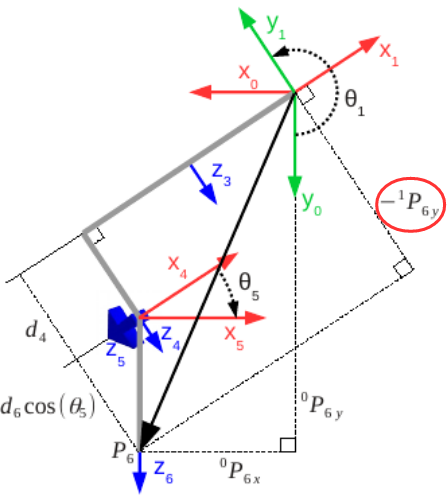
\includegraphics[width=0.5\textwidth]{Design/06.png}
    \caption{Angles and lengths of P61 \cite{Rasmus}} 
    \label{fig:rasmus2} 
\end{figure}

Inspecting figure \ref{fig:rasmus2}, another right-angled triangle can be found.\\
Excluding $_1^0T$, a new matrice can then be examined: $_6^1T$. 
Using the y, which is $^{-1}P_{6y}$, can be looked upon as $d_4+d_6\cdot\cos{\theta_5}$.
$^1P_6$ can then be expressed as the rotation of $^0P_6$ around $z_1$, where the y's are expressed as $\sin{\theta_1}and\cos{\theta_1}$.
By using the transformation matrice $_6^0T$, see \ref{fig:transfomationM}, we can then use the arccos, which is the value of the x and y and then add it into the equation.\\
Using the left-hand rule the $\theta_5$ can stand alone and the equation will look like this:\\
(Expected outcome is 50 degrees.)\\
\begin{equation}
\centering
\large\theta_1 =\frac{arccos\cdot\frac{(-521.411\cdot Sin(\theta_1)-(-256.142)\cdot Cos(\theta_1)-d_4}{d_6}\cdot 180}{\pi}=49.99995
\end{equation}\\


\paragraph{Step 5:} Find theta 6.\\

The group found theta 6 by combining the different parameters from the rotation matrix, see \ref{fig:rotmat}.\\
The x and y parameters was used and then the tangent of the two parameters was found and inserted in the equation of theta 6.
The result was expected to be 60 degrees.\\

\begin{equation}
\centering
\theta_6 = \frac{^1_2 P}{\pi} \cdot 180 = 59.999999999
\label{}
\end{equation}\\

Knowing that the x and y parameters is considered a rotation by sine to theta 1, the sine and cosines were placed behind the parameters, respectively sin after x and cos after y, and lastly divided with the sine to theta 5.

\paragraph{Step 6:} Find theta 2,3 and 4.\\

The following thetas are parallel and can be reviewed in the attached maple document.\\


\section{Trajectories}
When the angle degrees is known from inverse kinematics to two given positions, it is possible to calculate the trajectories. The purpose of planning the trajectories of the robot manipulator, is to control the trajectory. This makes the acceleration of the manipulators joints more smooth.\\
Doing so will make the movements predictable and accurate, and should help avoiding the singularity problem \cite{Trajectory}. 


\subsection{Joint trajectories}

Using joint trajectories, 3 categories have to be determined:\\
Position, Velocity and Acceleration.
These three polynomials can be described as the trajectory.\\
In this section we denote the following:
\begin{equation}
    a_0 =\theta_{start} 
\end{equation}
\begin{equation}
    a_1 = \omega_{start}
\end{equation}
\begin{equation}
    a_2 = \frac{3}{t_{finish}} \cdot (\theta_{end} - \theta_{start})
\end{equation}
\begin{equation}
    a_3 = \frac{-2}{t_{finish}} \cdot (\theta_{end} - \theta_{start})
\end{equation}
The position a is computed by \(\theta(t)\), which is described as: \[\theta(t)=a_0+a_1t+a_2t^2+a_3t^3\]
This function can be used to describe the velocity and acceleration by using its derivatives\cite{JointTrajectories}:\[\Dot{\theta}(t)\] and \[\Ddot{\theta}(t)\]

\subsection{Joint position}
In figure \ref{fig:position2} we are showing the rotational movements of the 6 joints on the UR5, when it is performing the task of moving the rotor from the conveyor belt, to the balancing machine.\\
For each joint it is calculated using the formula: 
\begin{equation}
  \theta(t)=a_0+a_1t+a_2t^2+a_3t^3
\end{equation}

\subsection{Joint velocity}
In figure \ref{fig:velocity2} we calculate the movement speed of the 6 joints, we do this by using the derivative of the position formula, which then becomes
\begin{equation}
\Dot{\theta}(t)=a_1+2a_2t+3a_3t^2
\end{equation}

\subsection{Joint Acceleration}
In figure \ref{fig:acceleration} the acceleration of the 6 joints are calculated based on the joint position change, this is done by taking the double derivative of the position change formula, which then becomes:
\begin{equation}
\Ddot{\theta}(t)=2a_2+6a_3t
\end{equation}

\subsubsection{From point 1: "Conveyor" to point 2: "Balancing", where t is from 0 to 2.6}

\begin{figure}[H]
  \centering
  \begin{minipage}[b]{0.45\textwidth}
    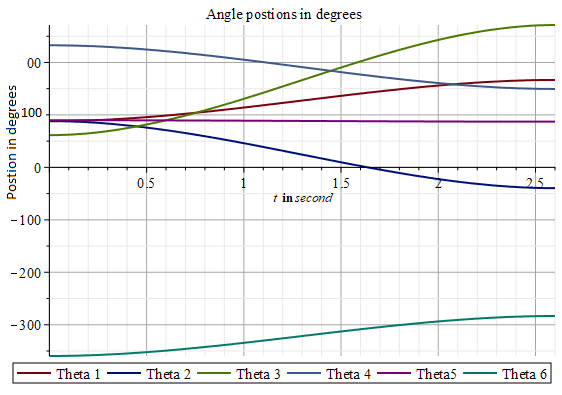
\includegraphics[width=\textwidth]{Design/poscb.png}
    \caption{Position for point 1 to 2}
    \label{fig:position2}
  \end{minipage}
  \hfill
  \begin{minipage}[b]{0.45\textwidth}
    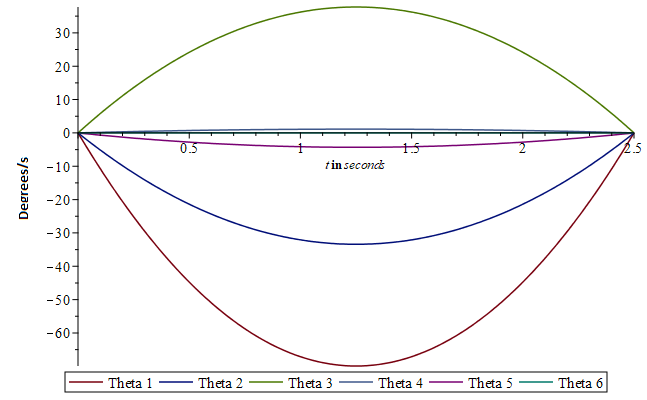
\includegraphics[width=\textwidth]{Design/velcb.png}
    \caption{Velocity for point 1 to 2}
    \label{fig:velocity2}
  \end{minipage}
\end{figure}
\begin{figure}[H]
  \centering
  \begin{minipage}[b]{0.45\textwidth}
    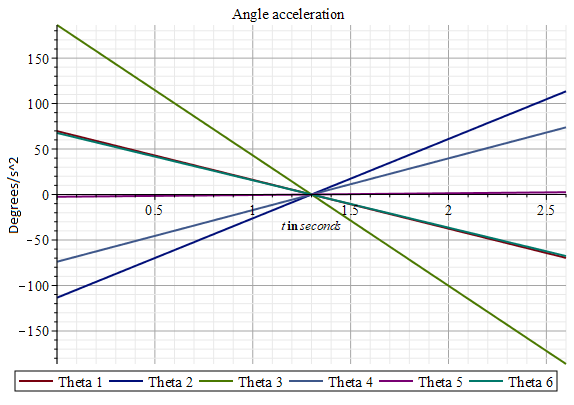
\includegraphics[width=\textwidth]{Design/acccb.png}
    \caption{Acceleration for point 1 to 2}
    \label{fig:acceleration}
   \end{minipage}
\end{figure}
 
\section{Conclusion}
Describing a robot with forward kinematics and Denavit-Hartenberg parameters is used to locate the different joints and the tool in a 3D-space, so the robot can be manipulated and used for various tasks.\\
Looking at Denavit-Hartenberg, the advantage of this method is to simplify the different axis in a matrix, so the operator and the robot can identify where the different coordinate systems are located.\\
Forward kinematics is the starting point of selecting the DH-parameters, when we know the point $Z_{i-1}$ and $Z_1$ we can then locate every axis in the desired robot. Hereby conclude to DH-parameters and include them in to inverse kinematics.\\
Inverse kinematics are used to find the different angles of the robot, so that it can be fully investigated and used in trajectories.\\ 
When finding the angles of a 6 DOF robot, a lot of steps needs to be taken in to consideration. The thetas 1,5 and 6 can only be found by investigating the rotation matrice from forward kinematics, and inspecting the different angles and joints of the different posistions. While the thetas 2,3 and 4 can be looked upon as RRR parallels.\\
The trajectories relies solely on the inverse kinematics, since it uses the different thetas and joints to investigate the posistion, velocity and acceleration. These graphs are a huge part of the investigation of how our robot moves.\\
To conclude, the investigation of forward and inverse kinematic can be led in to parameters, that is used in the calculation of the movements of the manipulator.\\






